\documentclass{jarticle}
\usepackage{robomech}
\usepackage[dvipdfmx]{graphicx}
\usepackage{amsfonts}
\usepackage{hyperref}

\begin{document}
\makeatletter
\title{価値反復を用いた移動ロボットによる屋外ナビゲーション}
{}
{Outdoor navigation with a mobile robot using value iteration}
{}

\author{
	\begin{tabular}{ll}
		○学\hspace{1zw}登内 リオン(千葉工大)& 正\hspace{1zw}林原 靖男\hspace{1zw} (千葉工大)\\
 		\hspace{1zw}正\hspace{1zw}上田 隆一(千葉工大)\\
		% ※協賛・後援団体の会員資格で発表される場合は「正・学」は不要です。
	\end{tabular}
	% &\\
	\vspace{1zh} \\
	\begin{tabular}{l}
			{\small Leon TONOUCHI, Chiba Institute of Technology, s20c1078un@s.chibakoudai.jp} \\
			{\small Ryuichi UEDA, Chiba Institute of Technology} \\
			{\small Yasuo HAYASHIBARA, Chiba Institute of Technology}             \\
	\end{tabular}
}
\makeatother

\abstract{ \small
We examine our software package for mobile robot navigation in the real world. 
This software uses value iteration for updating a decision making policy 
in the whole state space. Though the computational cost of this method
is too large for current computers, we expect that it will be standard
in future. In the experiments, we use this package with a laptop computer on
a mobile robot. Though the calculation time is still a problem,  
it works on the mobile robot for the first time. 
}

\date{} % 日付を出力しない
\keywords{robot navigation, brute-force value iteration}

\maketitle
\thispagestyle{empty}
\pagestyle{empty}

\small
\section{緒言}%===========================
%本文:明朝体・9pt(欧文Times New Roman, 9pt)、文字間隔は1行26文字程度、行間隔は4.2mm程度にして下さい。
価値反復は、ベルマン最適方程式を用いて、 
有限マルコフ決定過程における最適方策を正確に求めることができる手法である\cite{Shinjuku1}。
価値反復を移動ロボットの行動計画に適用すると、
環境中でロボットがとりうる全ての位置と向きに対して、最適な行動を計算できる\cite{上田robosym2022}。
しかし、経路計画によく用いられるA*\cite{Shinjuku3}などの探索手法よりも、
計算量が大きい。
だが、計算機の性能向上でその問題が将来的に小さくなると、
探索手法よりも優れた解が得られ、
予期せぬ障害物に対しても、より効率のよい迂回経路を示すことができる。

上田らは、現在の計算機でも、
限られた環境の広さであれば価値反復を利用できるのではないかと考え、
価値反復による経路計画のためのROSパッケージを実装した\cite{上田rsj2021}。
シミュレーション中では、100$\mathrm{[m^2]}$超の環境において、
ハイエンドのノートパソコンで3秒程度の計算コストで
計画可能であることを示した。
しかし、パッケージ自体が実際の移動ロボットで試されたことはない。
実際の移動ロボットでは搭載できるノートパソコンの大きさや
利用できる電力に制限があり、
また、計算能力に余力がないと、ロボットの動作が不安定になる可能性がある。


そこで本稿では、このパッケージを屋外移動ロボットで用い、
実機がこのパッケージで実際にナビゲーション可能かどうかと、
実環境での計算量を調査する。
2章で今回行った実験の環境や結果, 実験に用いるROSパッケージについて説明し、
3章では結言を述べる。

%※ 講演番号、講演会名、ページ番号は記載しないようにして下さい。
\section{実装}%===========================

\subsection{価値反復ROSパッケージの実機への適用}

今回の実験では上田らが開発した価値反復ROSパッケージ
(\url{https://github.com/ryuichiueda/value_iteration}のコミット\texttt{22422bc}\dots)
\cite{上田rsj2021}をアールティ社のRaspberry Pi Catに適用した。
Raspberry Pi Catに、図\ref{fig:raspicat}のように
ノート型の計算機(ノートPC)を搭載し、
このノートPCのなかで、価値反復パッケージによる計算や、
自己位置推定などを実行する。
自己位置推定は、図中の2D LiDARで行う。
ノートPCは、CPUとしてIntel Core i7-11800H(8コア16スレッド)、
DRAMとしてDDR4-3200 64GBを持つノート型パソコン(ノートPC)
を搭載している。
今回の実験は、価値反復ROSパッケージが実機でナビゲーション
可能かどうかを調査する目的があるため、パッケージに変更は加えなかった。
ロボットのとれる速度、角速度の組み合わせ(行動)も、
\cite{上田rsj2021}と同じく6種類のままとした。
これらの行動を表\ref{table:actions}に示す。

\begin{figure}[htb]
  \centering
   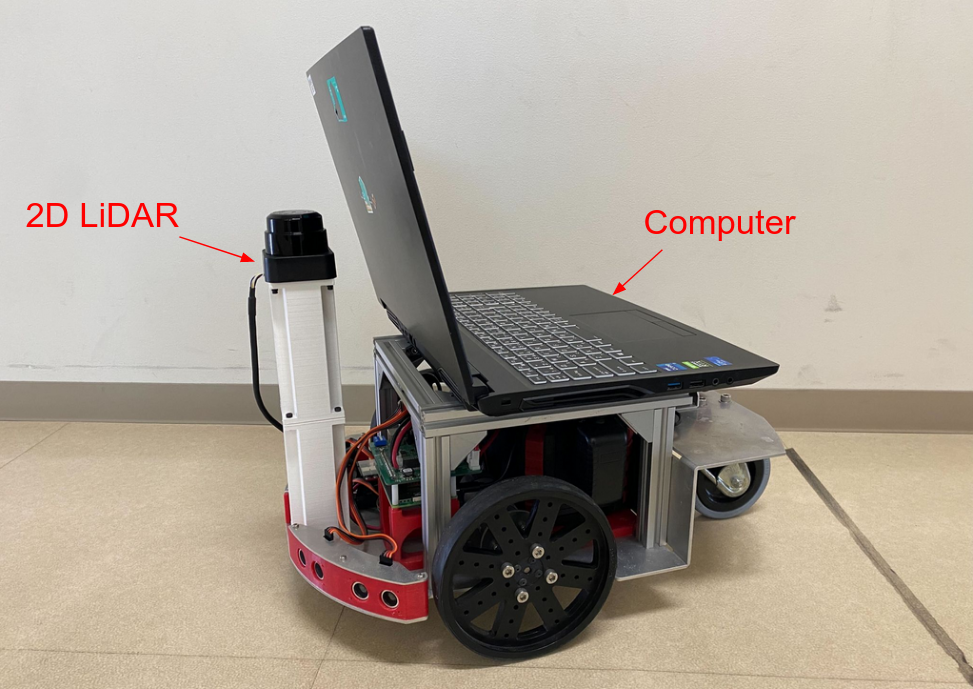
\includegraphics[height=55mm]{./figs/raspicat.png}
   \caption{Experimental setup}
	\label{fig:raspicat}
\end{figure}

\begin{table}[hbtp]
	\caption{Actions}
	\label{table:actions}
	\centering
	\begin{small}
	\begin{tabular}{l|cc}
 		\hline
		& forward & angular \\
 		type & verosity[m/s] & verosity[deg/s] \\
 		\hline \hline
 		forward & 0.3 & 0.0 \\
 		backward & -0.2 & 0.0 \\
 		right & 0.0 & -20.0 \\
 		left & 0.0 & 20.0 \\
 		right forward & 0.2 & -20.0 \\
 		left forward & 0.2 & 20.0 \\
	 \hline
	\end{tabular}
	\end{small}
\end{table}


\subsection{環境と地図}

Raspberry Pi Catを走らせる環境は、
千葉工業大学津田沼キャンパスの敷地とした。
この環境を走らせるために、
図\ref{fig:tsudanuma}の地図を準備した。
形式は、ROSのナビゲーションスタックで用いられる
画像形式の占有格子地図であり、白色が
障害物のない画素、黒色が障害物のある画素、
灰色が不明な画素を表す。

\begin{figure}[htb]
  \centering
   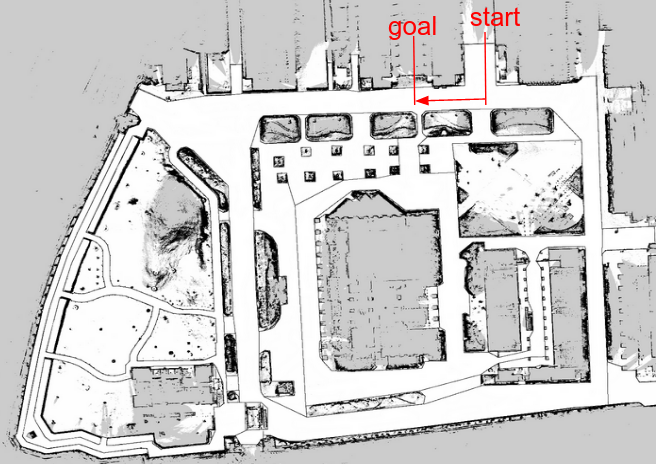
\includegraphics[height=55mm]{./figs/tsudanuma.png}
   \caption{the map for value iteration}
	\label{fig:tsudanuma}
\end{figure}

この地図のパラメータ等を
表\ref{table:map}に示す。
画素数は幅1,962[pixel]、
高さ1,333[pixel]で、
1画素あたりの解像度は幅、高さとも150[mm]である。
計算量に大きく関係する白色の画素の面積は
$3.7\times 10^3$[m$^2$]と、\cite{上田rsj2021}
の実験の30倍を超える。

表\ref{table:cells}は価値反復のために、
地図の$XY$平面に加えてロボットの向き$\theta$
も離散化して作った離散状態の数を示したものである。
$\theta$軸は6[deg]ごとに60分割したので、
離散状態数は表\ref{table:map}の値の60倍となる。
結果、障害物のない離散状態数は990万個となった。

\begin{table}[bth]
  \caption{configurations of the map}
	\label{table:map}
  \centering
	\begin{small}
  \begin{tabular}{l|r}
    \hline
    map size & 294.3 $\mathrm{[m]}\times 199.95\mathrm{[m]}$\\
    cell resolution &  0.15$\mathrm{[m]}\times 0.15\mathrm{[m]}$ \\
		number of cells & 2,615,346\\
    number of free cells & 165,076\\
		the area of the free cells & 3714.98$\mathrm{[m^2]}$\\
    \hline
  \end{tabular}
	\end{small}
	\caption{parameters for value iterations}
	\label{table:cells}
  \centering
  \begin{tabular}{l|r}
    \hline
    number of states & 156,920,760\\
    number of free states &  9,904,560\\
		number of actions & 6\\
    \hline
  \end{tabular}
\end{table}

\section{実験}%===========================

\subsection{評価実験}
まず、地図の大きさと比較して短い区間の移動を10回試行し、
価値反復の計算量を評価した。
また、ロボットが負荷の高い価値反復の計算をしながら
安定して走行できるか確認した。
走行区間は、図\ref{fig:tsudanuma}にあるスタート地点から
ゴール地点で、距離は$15.6$[m]である。
自己位置推定には上田が作成したROSのemclパッケージ
(\url{https://github.com/ryuichiueda/emcl})を用いた。

\begin{figure}[htb]
  \centering
   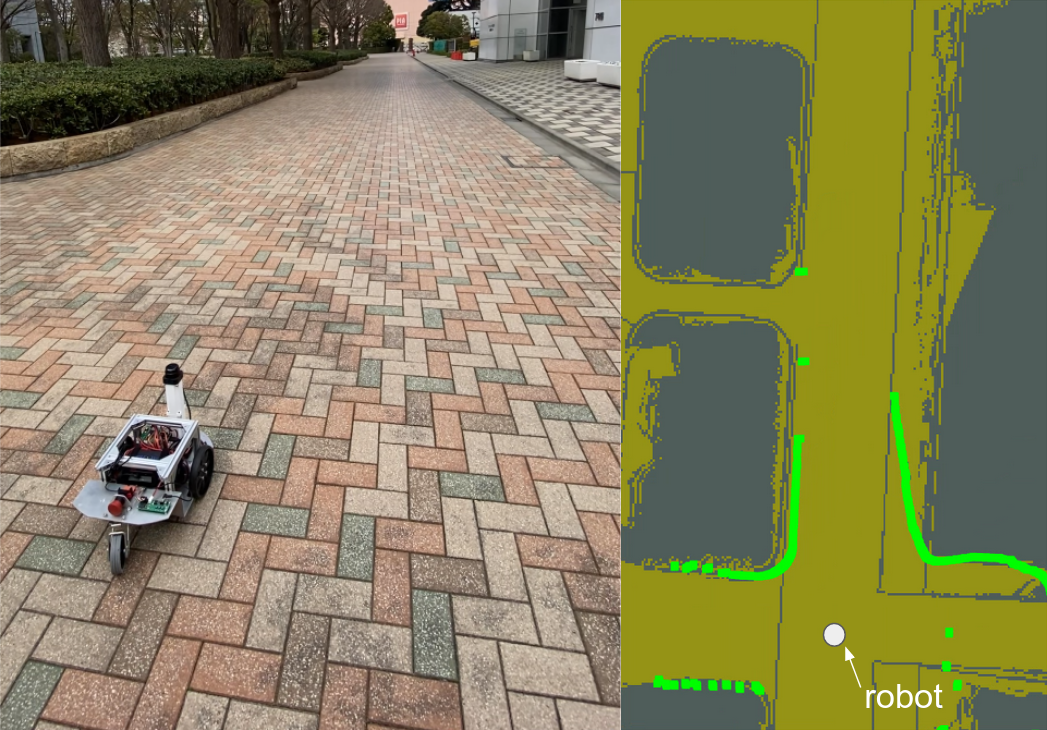
\includegraphics[height=61mm]{./figs/raspicat-start.png}
   \caption{Before goal installation}
	\label{fig:raspicat-start}
\end{figure}

図\ref{fig:raspicat-start}のように、
スタート地点に置かれたロボットは、
ゴール地点を予め指示されておらず、
図\ref{fig:raspicat-no-local}のように、
ゴール地点を指示されてから移動と価値反復を同時に行う。
ゴール地点を指示されてから、
ゴール地点にロボットが達するまでの時間を試行の所要時間とする。

\begin{figure}[htb]
  \centering
   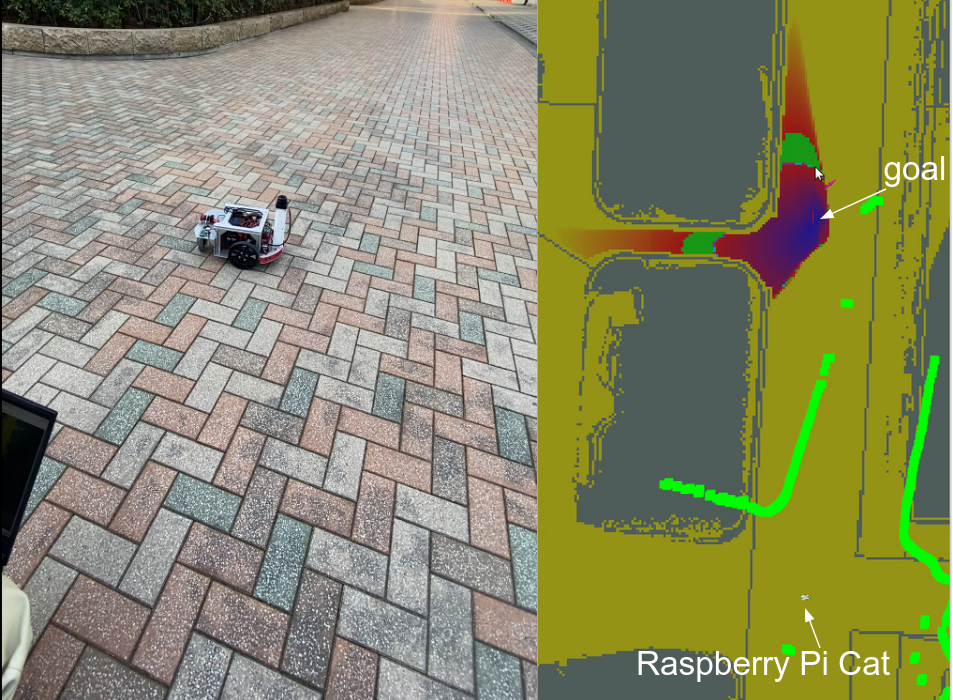
\includegraphics[height=55mm]{./figs/raspicat-no-local.png}
   \caption{setting the goal on online}
	\label{fig:raspicat-no-local}
\end{figure}

計算量の評価のために、
図\ref{fig:raspicat-after-planning}のように、
価値反復が終了して最適解が得られたあとに、
ロボットをスタート地点からゴール地点まで走らせる
試行も10回行った。
\begin{figure}[htb]
  \centering
   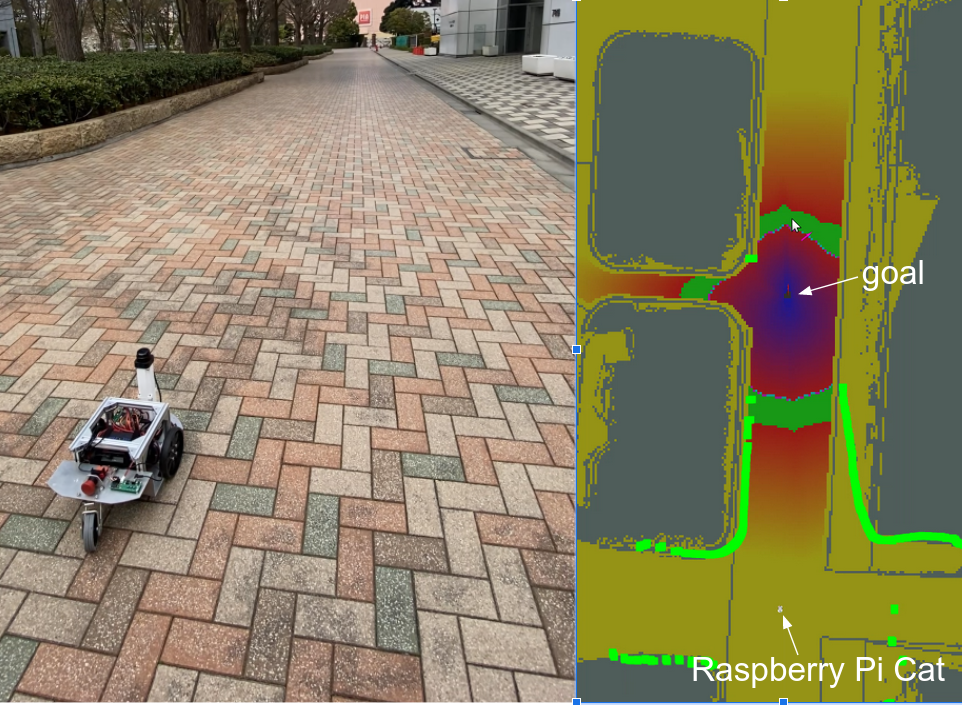
\includegraphics[height=55mm]{./figs/raspicat-after-planning.png}
   \caption{setting the goal on offline}
	\label{fig:raspicat-after-planning}
\end{figure}
この試行(オフライン計算を用いる試行)の時間を、
上記のスタートと同時に計算を開始する試行(オンライン計算を用いる試行)
から引くと、オンラインで計算にかかった実質的な時間となる。

\begin{table}[hbtp]
	\caption{computational complexity}
	\label{table:result}
	\centering
	\begin{small}
	 \begin{tabular}{l|cc}
		\hline
		 & average & standard \\
		 & of total time[s] & deviation[s] \\
		\hline \hline
		with online calculation & 123.3 & 6.2 \\
		after offline calculation &\ \ 89.6 & 3.4 \\
		\hline
		 difference & \ \ 33.7 & - \\
		\hline
	 \end{tabular}
	\end{small}
\end{table}

試行結果を表\ref{table:result}に示す。
表のように、オンライン計算とオフライン計算での
所要時間の差は$33.7$[s]であった。

この計算時間は、A*などを用いる方法と比較して
桁違いに遅いものとなった。
一方で、地図の解像度を落とすとこれよりも
計算量が小さくなる。
ただし、解像度とロボットの経路の最適性については
トレードオフの関係があるので、
今後調査の必要がある。

ロボットの挙動については、特に乱れるということはなかった。
オンライン計算の場合、
ロボットは最初目的地に向かわない挙動を示すが、
それ以外には、オンライン計算での試行と
オフライン計算での試行で、ロボットの挙動に大きな違いは見られなかった。

\subsection{追加実験}

追加の実験として長距離を走行させた場合の計算量を評価した。
図\ref{fig:tsudanuma-long-path}にあるスタートからゴールまで走行区間は$158.1$[m]である。
今回はスタート地点からゴール地点まで走らせる試行を、
オンライン計算の場合とオフライン計算の場合で1回ずつ行った。

\begin{figure}[htb]
  \centering
   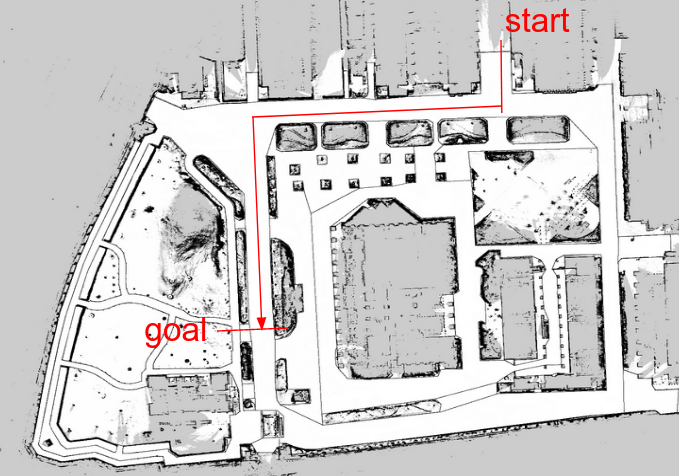
\includegraphics[height=55mm]{./figs/tsudanuma-long.png}
   \caption{the goal and path}
	\label{fig:tsudanuma-long-path}
\end{figure}

結果は表\ref{table:result2}に示す。
表のようにオンライン計算とオフライン計算での
所要時間の差は$35.1$[s]であった。
走行距離を伸ばした場合でも、計算量はほとんど変わらなかった。

\begin{table}[hbtp]
	\caption{computational complexity}
	\label{table:result2}
	\centering
	\begin{small}
	 \begin{tabular}{l|c}
		\hline
		 & total time[s] \\
		\hline \hline
		with online calculation & 613.6 \\
		after offline calculation & 578.5 \\
		\hline
		 difference & \ \ 35.1 \\
		\hline
	 \end{tabular}
	\end{small}
\end{table}

\section{結言}%===========================

本稿では、価値反復ROSパッケージを実ロボットで用い、
屋外の実環境を走行させた。
これまでシミュレーションでのみ動作が確認されていた同パッケージが、
実機でも動作することを確認した。
計算量については、$3714.98$[m$^2$]のフリースペースがある環境において、
$15.6$[m]の移動に対してIntel Core i7-11800Hで
$33.6$[s]の計算コストがかかるというものであった。
この計算コストについては、今後の計算機の性能の向上や、
地図の解像度の最適化などで改善されると考えられる。

\footnotesize
\begin{thebibliography}{99}

	\bibitem{Shinjuku1}
	Bellman, R., {\it Dynamic Programming}, Princeton Uni-versity Press, Princeton, NJ, 1957.

	\bibitem{上田robosym2022}
	上田隆一,池邉龍宏,林原靖男,``移動ロボットのナビゲーションのためのbrute-forceな価値反復を用いた大域計画・局所計画アルゴリズム'', 
	第27回ロボティクスシンポジア講演論文集, pp. 109-112, 2022.
	
	\bibitem{Shinjuku3}
	Hart, P. E., Nilsson, N. J. and Raphael, B. ``A Formal
	Basis for the Heuristic Determination of Minimal Cost
	Paths,'' {\it IEEE Transactions on Systems Science and Cybernetics}, Vol. 4, No. 2, pp. 100-107, 1968.
	
	\bibitem{上田rsj2021}
	上田隆一,池邉龍宏,林原靖男,``brute-forceな価値反復を用いた実時間経路計画ROSパッケージ'', 
	第39回日本ロボット学会学術講演会予稿集, RSJ2021AC2I1-04, 2021.

	\bibitem{上田rsj2022}
	上田隆一,池邉龍宏,林原靖男,``価値反復による準静的な障害物を考慮した実時間経路'', 
	第40回日本ロボット学会学術講演会予稿集, RSJ2022ACI2I2-01, 2022.

	\bibitem{上田robosym2023}
	上田隆一,登内リオン, 池邉龍宏,林原靖男,``移動ロボットのための自己位置の不確かさを考慮したセンシングできない固定障害物の回避方法'', 
	第28回ロボティクスシンポジア講演論文集, pp. 118-123 2023.

\end{thebibliography}

\normalsize
\end{document}
